% !TEX root = hazelnut-dynamics.tex

\subsection{Example 4: Type Holes and Dynamic Type Errors}
\label{sec:dynamic-type-errors}

% \begin{subfigure}[t]{\textwidth}
\begin{figure}
\centering
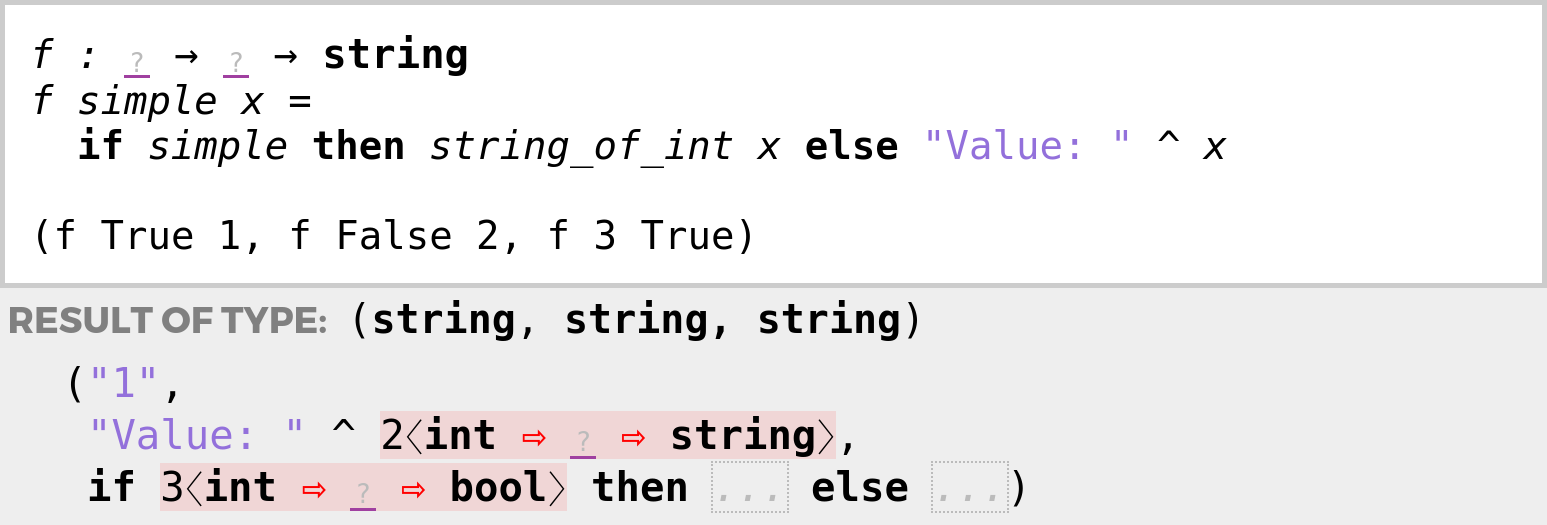
\includegraphics[width=0.71\textwidth,interpolate=false,valign=t]{images/cast-errors.png}
% 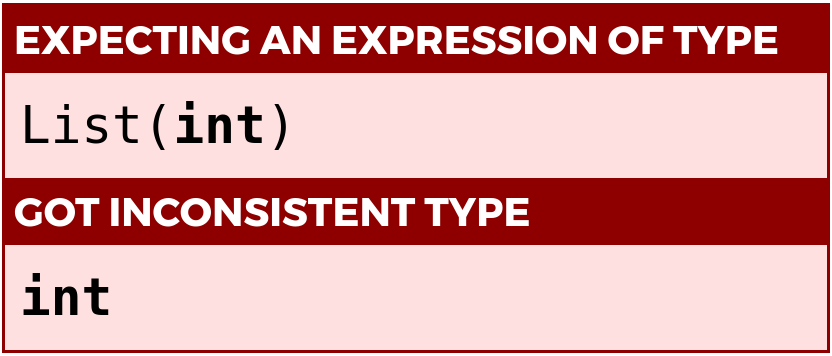
\includegraphics[width=0.28\textwidth,interpolate=false,valign=t]{images/type-inconsistency.png}
\caption{Example 4: Type Holes and Dynamic Type Errors}
\label{fig:cast-errors}
\vspace{-6px}
\end{figure}
% \end{subfigure}


% So far, we have only discussed incomplete programs where a hole appears within an expression.
In \Hazel, the program can also be incomplete because holes appear in types. 
\citet{popl-paper} confirmed that the literature on \emph{gradual type systems} \cite{Siek06a,DBLP:conf/snapl/SiekVCB15} is directly relevant to the problem of reasoning with type holes, by identifying the type hole with the unknown type. 
% Unsurprisingly, then, it is also relevant to the problem of running 
% programs with type holes. 
Indeed, the purpose of gradual typing is to be able to run programs that are not yet sufficiently annotated with types by inserting \emph{casts} only where necessary. As such, let us consider only a small synthetic example to demonstrate what is unique to our approach.

Fig.~\ref{fig:cast-errors} defines a simple function, \li{f}, of two arguments. 
The type annotation on the first line leaves the type of those arguments unknown. 
As such, the \Hazel type system, following the gradual typing approach,
allows the body of the function to use those two
arguments at any type (that is, the hole type is universally consistent). 
Here, the first argument, \li{simple}, is used at one type, \li{bool}, 
and the second argument, \li{x}, is used at two different types in the two branches (perhaps because the programmer made a mistake), 
 \li{int} and  \li{string}  ( \li{^} is string concatenation).
Although \Hazel supports only local type inference as of this writing, 
a system that uses ML-style type reconstruction to fill type holes statically, like GHC Haskell, would only be able to fill the first hole. Leaving the second hole unfilled is 
a parsimonious alternative to arbitrarily or heuristically choosing one of the possibilities and marking the
other uses of \li{x} as ill-typed (see \cite{DBLP:journals/jfp/ChenE18}).

At the bottom of the cell in Fig.~\ref{fig:cast-errors}, we have three 
example applications of \li{f}, tupled together for concision. All three are statically
well-typed, again because the hole type is universally consistent. 
The result at the bottom of Fig.~\ref{fig:cast-errors} demonstrates that the first application
of \li{f} is dynamically unproblematic. This allows the programmer to confirm that 
the first branch operates as intended without the need to 
address the typing problems in the other branch \cite{Bayne:2011:ASD:1985793.1985864}. 
% This flexibility is a common motivation for dynamic and gradual languages .

The second application of \li{f}, in contrast, causes a dynamic type error because the second argument, \li{2}, is an \li{int} but evaluation takes the branch where it is used as a \li{string}. 
Rather than aborting evaluation when this occurs, as in existing gradual type systems, the problematic term becomes a \emph{failed cast} term, shown shaded in red, which can be read ``\li{2} is an \li{int} that was used through a variable of hole type (\li{?}) as a \li{string}''. 
A failed cast acts much like a non-empty hole as a membrane around a problematic term. The surrounding concatenation operation becomes indeterminate, but  
evaluation can continue on to the third application of \li{f}, which is also problematic, this time because the first argument is not a \li{bool} (perhaps because the programmer had an incorrect understanding of the argument order). 
Again, this causes a failed cast to appear, this time in guard position. Like a hole in guard position, evaluation cannot determine which branch to take so the whole conditional becomes indeterminate. 
The pretty printer
hides the two branches behind ellipses for concision.

\ifarxiv

\else
In this small example, it might have only been a small burden for the programmer to provide the intended types in the signature for \li{f}, but there are situations (e.g. during rapid prototyping or a live performance) where the programmer might consider the burden more substantial. This approach ensures that dynamic feedback does not exhibit gaps even when there is a dynamic type error.
\fi


\begin{comment}
\emph{Gradual type systems}~(\eg{}~\cite{XXX,XXX,XXX}) can statically accept
programs that would otherwise be rejected by static type systems---either
because type inference cannot reconstruct a valid type assignment, or because
there may not be a unique valid type assignment at all.
%
In either case, gradual type systems allow types to contain \emph{unknown
types}, and partially unknown types can be used in contexts that require
different types, so long as they are \emph{consistent} (intuitively, equal
modulo the unknown parts).
%
Dynamic casts are then inserted to ensure that these remaining static
discrepancies are not violated at run-time.

\HazelnutLive{} inherits the notion of \emph{type holes} from
\citet{popl-paper}, which serves a similar static purpose as the unknown type in
gradual type systems.
%
In contrast to prior gradually typed languages, however, \HazelnutLive{} can
evaluate ``around'' cast errors in the same way as it does for expression holes.

\overviewExample{3}{Dynamically Typed Negation}

Consider the \li{negate} function (adapted from \cite{ChughPOPL2012}), which
cannot be assigned a static type in a conventional type system---either a
bidirectional one, like in \HazelnutLive{}, or one with ML-style,
unification-based inference---because the argument \li{x} is used at type
\li{int} on line \rkc{XXX} and \li{bool} on line \rkc{XXX}.
%
Therefore, the declared type of \li{x} is the hole type \li{??}, which allows
\li{x} to be used at the conflicting types, with each use expanded into an
expression wrapped in a \emph{cast} that will dynamically check for safety.
%
The return type also uses the hole type \li{??}, leading to additional casts in
the expansion.

\begin{lstlisting}
negate : bool -> ?? -> ??
negate b x =
  if b
    then 0 - x     // expanded to: (0 - (x<?? => int>))<int => ??>
    else not x     // expanded to: (not (x<?? => bool>))<bool => ??>

(negate false 1) + 2 + 3 + (negate true 4)
\end{lstlisting}

\noindent
%
As in prior gradually typed languages~\cite{XXX},
evaluating the expression \li{negate false 1} on line \rkc{XXX} leads to
\li{(not (1<int => ??><?? => bool>))<bool => ??>}, where the inner casts
lead to the \emph{cast error} \li{1<?? =/=> bool>} because \li{1} cannot be
safely treated as having type \li{bool}.
%
Unlike in prior gradually typed languages, however, \HazelnutLive{} evaluates
around the cast error, making progress on the \li{2 + 3 + negate false 4}
expression that surrounds the error; the final indeterminate result is
\li{(not (1<?? =/=> bool>))<bool => ??> + 1}.
%
Just like it is useful for static type checkers to report multiple errors, our
approach allows us to report multiple dynamic cast errors, and otherwise make
progress on expressions that do not depend on failed casts.
%
This approach can be incorporated into existing gradually typed languages.
\end{comment}